\documentclass{beamer}

\usepackage[utf8]{inputenc}
\usepackage[english]{babel}
\usepackage{graphicx}
\usepackage{color}
\usepackage{natbib}
\usepackage{amssymb}
\usepackage{amsmath}
\usepackage{algorithm}
\usepackage{algpseudocode}
\usepackage{caption}
\usepackage{euler}
\usepackage{tikz}
\usetikzlibrary{arrows,calc,tikzmark,shapes.misc}

\tikzset{every picture/.style=remember picture}
% Define a TikZ node for math content:
\newcommand{\mathnode}[2]{%
  \mathord{\tikz[baseline=(#1.base), inner sep = 0pt]{\node (#1) {$#2$};}}}

\DeclareMathOperator*{\argmin}{arg\,min}
\DeclareMathOperator*{\argmax}{arg\,max}

\newcommand{\gilles}[1]{\textcolor{red}{{\it GL: #1}}}


% Beamer layout
\hypersetup{colorlinks=True, citecolor=green, linkcolor=blue}

\let\oldbibitem=\bibitem
\renewcommand{\bibitem}[2][]{\label{#2}\oldbibitem[#1]{#2}}
\let\oldcite=\cite
\renewcommand\cite[1]{\hyperlink{#1}{\oldcite{#1}}}
\let\oldcitep=\citep
\renewcommand\citep[1]{\hyperlink{#1}{\oldcitep{#1}}}
\let\oldciteauthor=\citeauthor
\renewcommand\citeauthor[1]{\hyperlink{#1}{\oldciteauthor{#1}}}

\usetheme{boxes}
\beamertemplatenavigationsymbolsempty
\setbeamertemplate{sections/subsections in toc}[circle]
\setbeamertemplate{footline}[frame number]
\setbeamertemplate{itemize items}[circle]
\setbeamertemplate{itemize subitem}[square]

% Front slide
\title{{\bf QCD-aware Recursive Neural Networks \\
for Jet Physics}\\
\href{https://arxiv.org/abs/1702.00748}{arXiv:1702.00748}}
\author{{\it Gilles Louppe}, Kyunghyun Cho, Cyril Becot, Kyle Cranmer}
%\date{December 15, 2016}
\date{}

\tikzset{
  invisible/.style={opacity=0},
  visible on/.style={alt={#1{}{invisible}}},
  alt/.code args={<#1>#2#3}{%
    \alt<#1>{\pgfkeysalso{#2}}{\pgfkeysalso{#3}} % \pgfkeysalso doesn't change the path
  },
}

\begin{document}

\begin{frame}[plain]
\titlepage
\centering

\includegraphics[height=1.5em]{figures/nyu.jpg}
\end{frame}



% ==============================================================================

\begin{frame}
    \frametitle{A machine learning perspective}

    Kyle's talks on QCD-aware recursive nets:

    \begin{columns}
        \begin{column}{0.7\textwidth}
            {\footnotesize
            \begin{itemize}
                \item Theory Colloquium, CERN, May 24, \url{https://indico.cern.ch/event/640111/}
                \item DS@HEP 2017, Fermilab, May 10, \url{https://indico.fnal.gov/conferenceDisplay.py?confId=13497}
                \item Jet substructure and jet-by-jet tagging, CERN, April 20, \url{https://indico.cern.ch/event/633469/}
                \item Statistics and ML forum, CERN, February 14, \url{https://indico.cern.ch/event/613874/contributions/2476427/}
            \end{itemize}}
        \end{column}
        \begin{column}{0.25\textwidth}
            \centering
            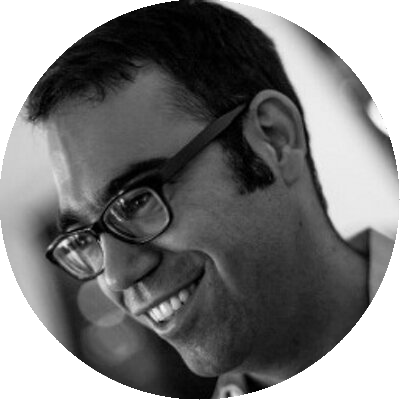
\includegraphics[width=\textwidth]{figures/kyle.png}
        \end{column}
    \end{columns}

    \vspace{0.5cm}

    Today: the inner mechanisms of recursive nets for jet physics.


\end{frame}

\begin{frame}
    \frametitle{Neural networks 101}

    \begin{columns}
        \begin{column}{0.65\textwidth}
                Goal = Function approximation
                \begin{itemize}
                    \item Learn a map from $x$ to $y$ based solely on observed pairs
                    \item Potentially non-linear map from $x$ to $y$
                    \item $x$ and $y$ are {\color{blue} fixed dimensional vectors}
                \end{itemize}

                \vspace{0.5cm}

                Model = Multi-layer perceptron (MLP)
                \begin{itemize}
                    \item Parameterized composition $f(\cdot; \theta)$ of non-linear transformations
                    \item Stacking transformation layers allows to learn (almost any) arbitrary highly non-linear mapping
                \end{itemize}
        \end{column}
        \begin{column}{0.4\textwidth}
            \centering
            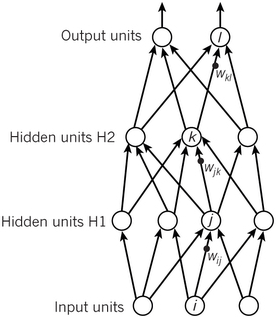
\includegraphics[width=\textwidth]{figures/nn1.png}
        \end{column}
    \end{columns}

    % goal = supervised learning
    % x and y and fixed dimensional real-valued vectors
    % model = Parameterized composition of non-linear activations

    \begin{tikzpicture}[remember picture,overlay]
        \node[left, yshift=-0.25cm] at (current page.north east) {\tiny Credits: \href{https://www.nature.com/nature/journal/v521/n7553/full/nature14539.html}{Lecun et al, 2015}};
    \end{tikzpicture}
\end{frame}

\begin{frame}
    \frametitle{Learning}

    \begin{itemize}
        \item Learning by optimization
        \item Cost function $$J(\theta; D) = \frac{1}{N} \sum_{i=1}^N \ell(y_i, f(x_i; \theta))$$
        \item Stochastic gradient descent optimization $$\theta_m := \theta_{m-1} - \eta \nabla_\theta J(\theta_{m-1}; B_m)$$
        where $B_m \in D$ is a random subset of $D$.

    \end{itemize}

    \vspace{0.5cm}

    \centering
    \it How does one derive  $\nabla_\theta J(\theta)$?

    % fig 6.11 + formula
    % nn =  data flow graphs
    % chain rule of calculus applied recursively from backward (2nd slide)

\end{frame}

\begin{frame}
    \frametitle{Computational graphs}

    \begin{align*}
        f(x; \theta=(W^{(1)}, W^{(2)})) &= W^{(2)} \texttt{relu}(W^{(1)}x) \quad~\text{(simplified 1-layer MLP)}\\
        J(\theta=(W^{(1)}, W^{(2)})) &= J_{MLE} + \lambda \left( \sum_{i,j} \left( W_{i,j}^{(1)} \right)^2 + \left( W_{i,j}^{(2)} \right)^2 \right)
    \end{align*}

    \begin{center}
        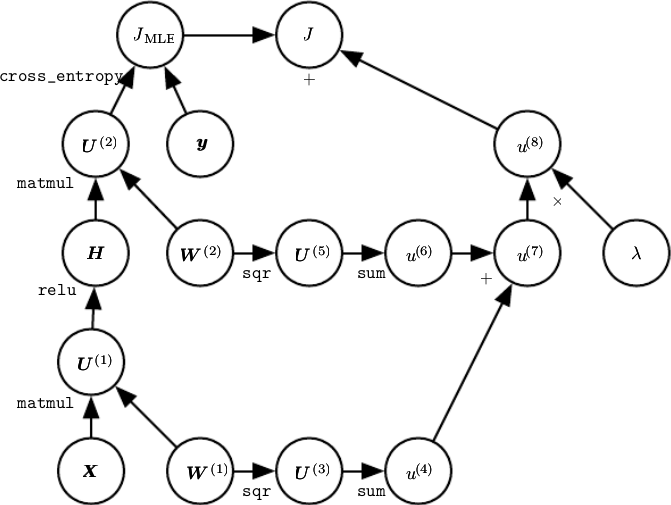
\includegraphics[width=0.65\textwidth]{figures/graph1.png}
    \end{center}


    % fig 6.11 + formula
    % nn =  data flow graphs
    % chain rule of calculus applied recursively from backward (2nd slide)

    \begin{tikzpicture}[remember picture,overlay]
        \node[left, yshift=-0.25cm] at (current page.north east) {\tiny Credits: \href{http://www.deeplearningbook.org/}{Goodfellow et al, 2016. Section 6.5.}};
    \end{tikzpicture}
\end{frame}

\begin{frame}
    \frametitle{Backpropagation}

    \begin{itemize}
        \item Backpropagation = Efficient computation of $\nabla_\theta J(\theta)$
        \item Implementation of the chain rule for the (total) derivatives
        \item Applied recursively from backward by walking the computational graph from outputs to inputs
    \end{itemize}

    \begin{columns}
        \begin{column}{0.5\textwidth}
            \begin{center}
                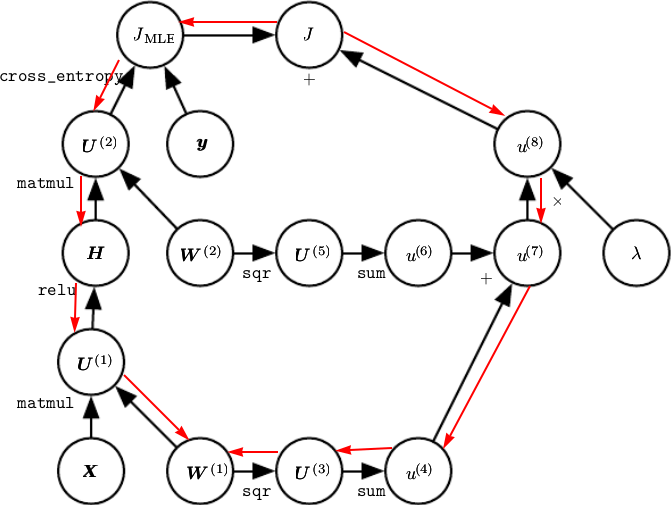
\includegraphics[width=\textwidth]{figures/graph2.png}
            \end{center}
        \end{column}
        \begin{column}{0.5\textwidth}
            \small
            \begin{align*}
                \frac{dJ}{dW^{(1)}} &= \frac{\partial J}{\partial J_{MLE}} \frac{d J_{MLE}}{dW^{(1)}} + \frac{\partial J}{\partial u^{(8)}} \frac{d u^{(8)}}{dW^{(1)}} \\
                \frac{d J_{MLE}}{dW^{(1)}} &= \dots \quad\text{(recursive case)}\\
                \frac{d u^{(8)}}{dW^{(1)}} &= \dots \quad\text{(recursive case)}
            \end{align*}
        \end{column}
    \end{columns}


    % fig 6.11 + formula
    % nn =  data flow graphs
    % chain rule of calculus applied recursively from backward (2nd slide)

\end{frame}

\begin{frame}
    \frametitle{Recurrent networks}

    \begin{columns}
        \begin{column}{0.75\textwidth}
            Setup
            \begin{itemize}
                \item {\color{blue} Sequence} $x = (x_1, x_2, ..., x_{\tau})$
                \begin{itemize}
                    \item E.g., a sentence given as a chain of words
                \end{itemize}
                \item The length of each sequence may vary
            \end{itemize}

            \vspace{0.5cm}

            Model = Recurrent network
            \begin{itemize}
                \item Compress $x$ into a single vector by recursively applying a MLP with shared weights on the sequence, then compute output.
                \item $h^{(t)} = f(h^{(t-1)}, x^{(t)}; \theta) $
                \item $o = g(h^{(\tau)}; \theta)$
            \end{itemize}
        \end{column}
        \begin{column}{0.2\textwidth}
            \centering
            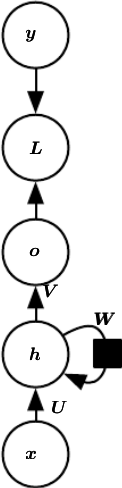
\includegraphics[scale=0.3]{figures/rnn1.png}
        \end{column}
    \end{columns}


    \vspace{0.5cm}

    \centering
    \it How does one backpropagate through the cycle?

    % x is a sequence
    % f is  a defined as a recurrence on this sequence
    % data flow graph

\end{frame}

\begin{frame}
    \frametitle{Backpropagation through time}

    \begin{itemize}
        \item Unroll the recurrent computational graph through time
        \item Backprop through this graph to derive gradients
    \end{itemize}

    \vspace{0.5cm}

    \begin{columns}
        \begin{column}{0.3\textwidth}
            \centering
            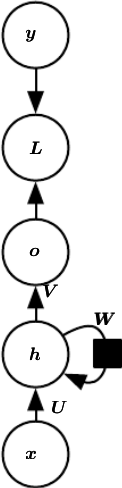
\includegraphics[scale=0.3]{figures/rnn1.png}
        \end{column}
        \begin{column}{0.1\textwidth}
            $\xrightarrow{\text{unroll}}$
        \end{column}
        \begin{column}{0.6\textwidth}
            \centering
            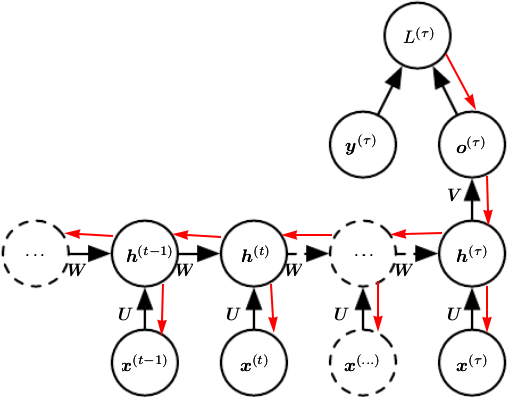
\includegraphics[scale=0.3]{figures/rnn2.png}
        \end{column}
    \end{columns}


    % unroll graph, then apply backprop
    % in two slides

    \begin{tikzpicture}[remember picture,overlay]
        \node[left, yshift=-0.25cm] at (current page.north east) {\tiny Credits: \href{http://www.deeplearningbook.org/}{Goodfellow et al, 2016. Section 10.2.}};
    \end{tikzpicture}
\end{frame}

\begin{frame}

    {\color{red}
    This principle generalizes to any kind of (recursive or iterative) computation that can be unrolled into a directed acyclic  computational graph.}

    \vspace{1cm}

    (That is, to any program!)
\end{frame}

\begin{frame}
    \frametitle{Recursive networks}

    \begin{columns}
        \begin{column}{0.75\textwidth}
            Setup
            \begin{itemize}
                \item  $x$ is structured as a {\color{blue} tree}
                \begin{itemize}
                    \item E.g., a sentence and its parse tree
                \end{itemize}
                \item The topology of each training input may vary
            \end{itemize}

            \vspace{0.5cm}

            Model = Recursive networks
            \begin{itemize}
                \item Compress $x$ into a single vector by recursively applying a MLP with shared weights on the tree, then compute output.
                \item $h^{(t)} = \begin{cases}
                        v(x^{(t)}; \theta) \quad\text{if $t$ is a leaf} \\
                        f(h^{(t_\text{left})}, h^{(t_\text{right})}; \theta) \quad\text{otherwise}
                    \end{cases}$
                \item $o = g(h^{(0)}; \theta)$
            \end{itemize}
        \end{column}
        \begin{column}{0.24\textwidth}
            \centering
            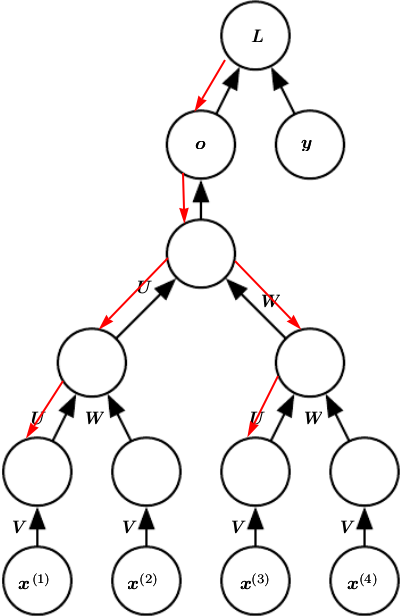
\includegraphics[scale=0.2]{figures/rnn3.png}
        \end{column}
    \end{columns}


    \begin{tikzpicture}[remember picture,overlay]
        \node[left, yshift=-0.25cm] at (current page.north east) {\tiny Credits: \href{http://www.deeplearningbook.org/}{Goodfellow et al, 2016. Section 10.6.}};
    \end{tikzpicture}
\end{frame}


\begin{frame}
    \frametitle{Dynamic computational graphs}

    \begin{itemize}
        \item Most frameworks (TensorFlow, Theano, Caffee or CNTK) assume a static computational graph.
        \item Reverse-mode auto-differentiation builds computational graphs dynamically on the fly, as code executes.

        \begin{itemize}
            \item One can change how the network behaves (e.g. depending on the input topology) arbitrarily with zero lag or overhead.
            \item Available in autograd, Chainer, PyTorch or DyNet.
        \end{itemize}
    \end{itemize}

    \centering
    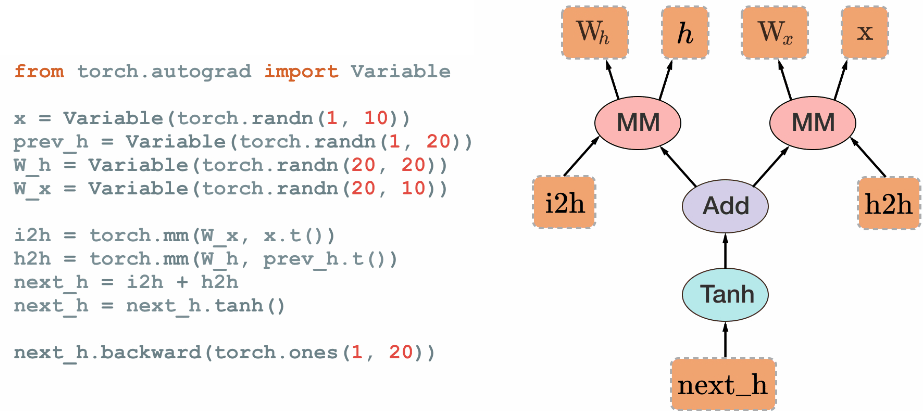
\includegraphics[scale=0.3]{figures/pytorch.png}


    \begin{tikzpicture}[remember picture,overlay]
        \node[left, yshift=-0.25cm] at (current page.north east) {\tiny Credits: \href{http://pytorch.org/about/}{pytorch.org/about}};
    \end{tikzpicture}
    % note on dynamic computational graphs
    % automated batchization
    % autograd dynet pytorch
\end{frame}


\begin{frame}
    \frametitle{Operation batching}

    \begin{itemize}
        \item Distinct per-sample topologies make it difficult to vectorize operations.
        \item However, in the case of trees, computations can be performed in batch level-wise, from bottom to top.
    \end{itemize}

    \vspace{1cm}

    \centering
    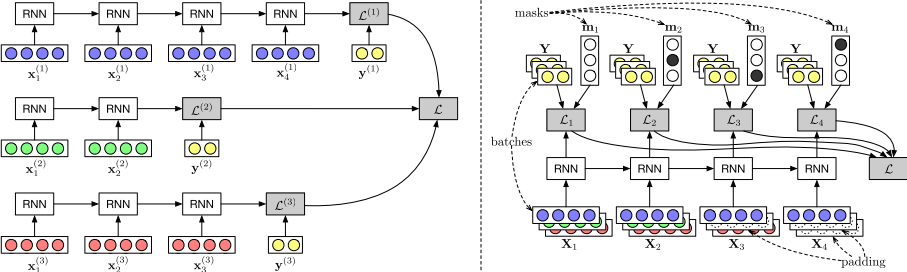
\includegraphics[width=\textwidth]{figures/batching.png}\\
    {\it On-the-fly operation batching (in DyNet)}


    \begin{tikzpicture}[remember picture,overlay]
        \node[left, yshift=-0.25cm] at (current page.north east) {\tiny Credits: \href{https://arxiv.org/abs/1705.07860}{Neubig et al, 2017}};
    \end{tikzpicture}
\end{frame}


\begin{frame}
    \frametitle{From sentences to jets}

    \begin{center}
        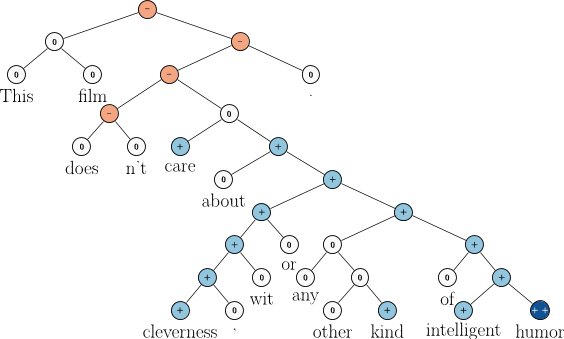
\includegraphics[width=0.8\textwidth]{figures/parse-tree.png}
    \end{center}


    Analogy:
    \begin{itemize}
        \item word $\rightarrow$ particle
        \item sentence $\rightarrow$ jet
        \item parsing $\rightarrow$ jet algorithm
    \end{itemize}
\end{frame}

\begin{frame}
    \frametitle{Jet topology}

    \begin{itemize}
        \item Use sequential recombination jet algorithms ($k_T$, anti-$k_T$, etc) to define computational graphs (on a per-jet basis).
        \item The root node in the graph provides a fixed-length embedding of a jet, which can then be fed to a classifier.
        \item Path towards ML models with good physics properties.
    \end{itemize}

    \vspace{0.5cm}

    \begin{center}
        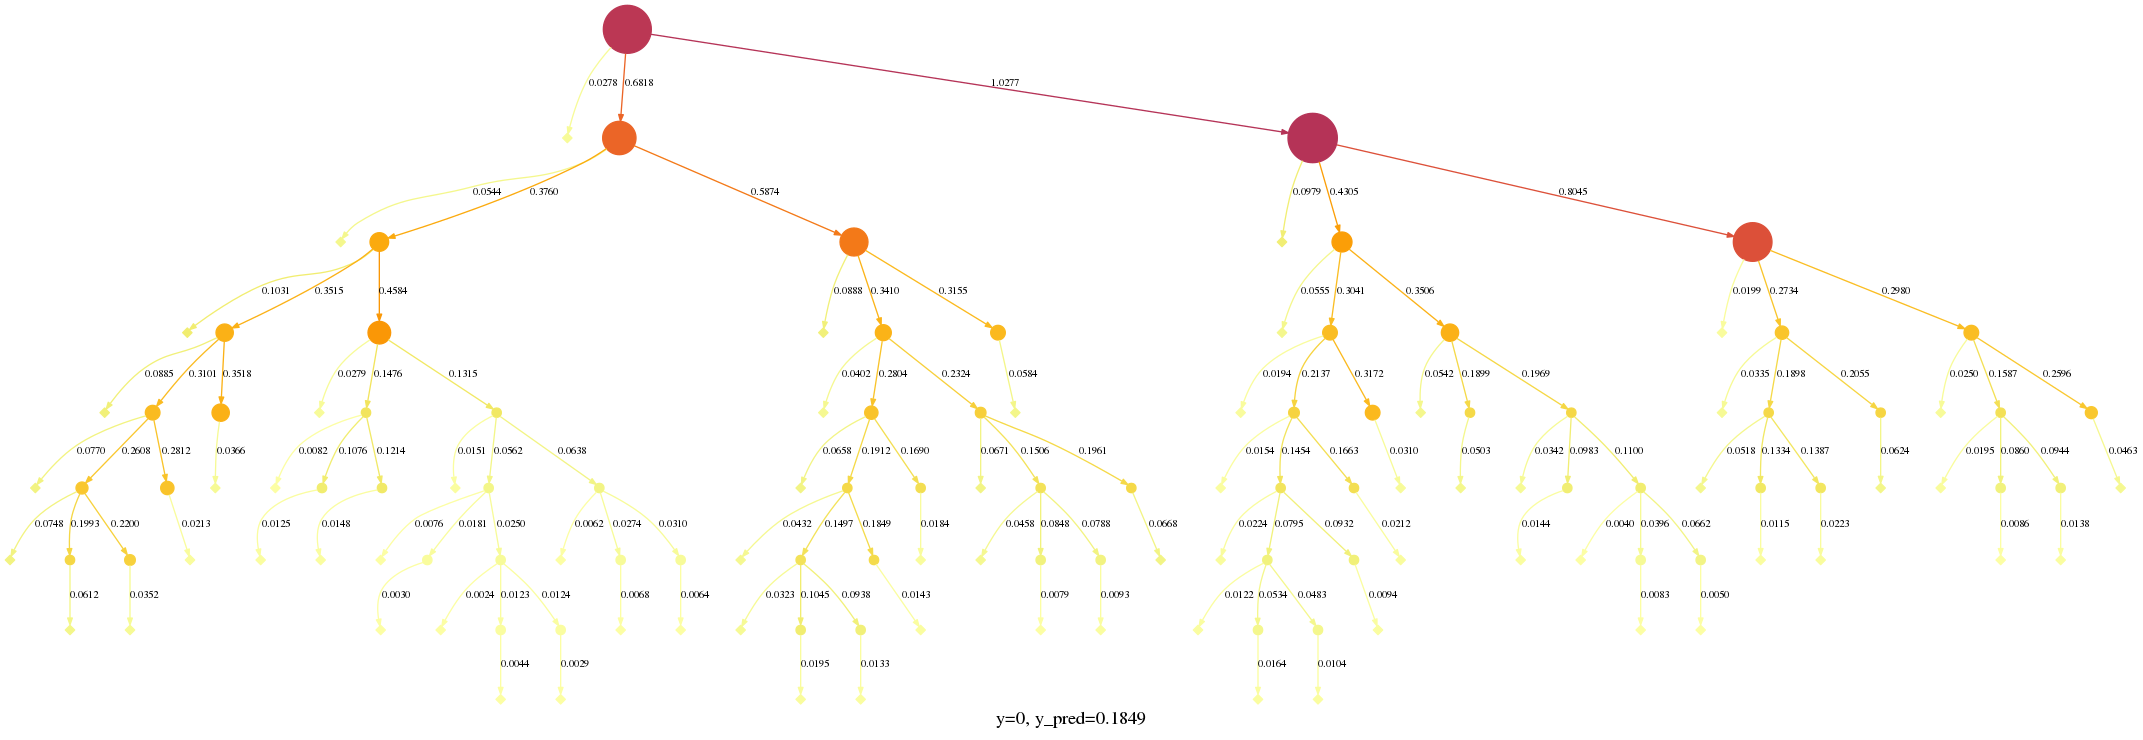
\includegraphics[width=0.8\textwidth]{figures/4320-kt.png}\\
        \it A jet structured as a tree by the $k_T$ recombination algorithm
    \end{center}
\end{frame}

\begin{frame}
    \frametitle{QCD-aware recursive neural networks}

    \vspace{-0.35cm}

    \begin{columns}
        \begin{column}{0.7\textwidth}
            \only<1>{{\it Simple recursive activation}:
            Each node $k$ combines a non-linear transformation $u_k$ of the 4-momentum $o_k$ with the left and right embeddings $h_{k_L}$ and $h_{k_R}$.

            {\tiny
            \begin{align*}
            \mathbf{h}^\text{jet}_k &=
             \begin{cases}
              \mathbf{u}_k          & \text{if } k \text{ is a leaf} \\
              \sigma \left( W_h
              \begin{bmatrix}
                  \mathbf{h}^\text{jet}_{k_L} \\
                  \mathbf{h}^\text{jet}_{k_R} \\
                  \mathbf{u}_k
              \end{bmatrix} + b_{h} \right)  & \text{otherwise}
             \end{cases} \label{eqn:rec-nn}\\
             %
             \mathbf{u}_k &= \sigma \left( W_u g(\mathbf{o}_k) + b_u \right) \\
             %
             \mathbf{o}_k &=
             \begin{cases}
             \mathbf{v}_{i(k)} & \text{if } k \text{ is a leaf} \\
             \mathbf{o}_{k_L} + \mathbf{o}_{k_R} & \text{otherwise}
             \end{cases}
         \end{align*}}
         }\only<2>{{\it Gated recursive activation}:
         Each node actively selects, merges or propagates up the left, right or local embeddings as enabled with reset and update gates $\mathbf{r}$ and $\mathbf{z}$.
         (Similar to a GRU.)

         {\tiny
         \begin{align*}
         \mathbf{h}^\text{jet}_k &=
          \begin{cases}
           \mathbf{u}_k & \text{if } k \text{ is a leaf} \\
           \mathbf{z}_H \odot \tilde{\mathbf{h}}^\text{jet}_k + \mathbf{z}_L \odot \mathbf{h}^\text{jet}_{k_L} +  & \text{otherwise}\\
           \hookrightarrow \mathbf{z}_R \odot \mathbf{h}^\text{jet}_{k_R}  + \mathbf{z}_N \odot \mathbf{u}_{k} &
          \end{cases} \label{eqn:rec-nn-gated}\\
         %
        %  \mathbf{u}_k &= \sigma \left( W_u g(\mathbf{o}_k) + b_u \right) \\
        %  %
        %  \mathbf{o}_k &=
        %  \begin{cases}
        %  \mathbf{v}_{i(k)} & \text{if } k \text{ is a leaf} \\
        %  \mathbf{o}_{k_L} + \mathbf{o}_{k_R} & \text{otherwise}
        %  \end{cases}\\
         %
         \tilde{\mathbf{h}}^\text{jet}_k &= \sigma \left( W_{\tilde{h}}
         \begin{bmatrix}
             \mathbf{r}_L \odot \mathbf{h}^\text{jet}_{k_L} \\
             \mathbf{r}_R \odot \mathbf{h}^\text{jet}_{k_R} \\
             \mathbf{r}_N \odot \mathbf{u}_{k}
         \end{bmatrix} + b_{\tilde{h}} \right)\\
         %
         \begin{bmatrix}
         \mathbf{z}_H \\
         \mathbf{z}_L \\
         \mathbf{z}_R \\
         \mathbf{z}_N
         \end{bmatrix} &= \text{softmax} \left( W_z
         \begin{bmatrix}
             \tilde{\mathbf{h}}^\text{jet}_k \\
             \mathbf{h}^\text{jet}_{k_L} \\
             \mathbf{h}^\text{jet}_{k_R} \\
             \mathbf{u}_{k}
         \end{bmatrix} + b_z
         \right) \\
         %
         \begin{bmatrix}
         \mathbf{r}_L \\
         \mathbf{r}_R \\
         \mathbf{r}_N
         \end{bmatrix} &= \text{sigmoid} \left( W_r
         \begin{bmatrix}
             \mathbf{h}^\text{jet}_{k_L} \\
             \mathbf{h}^\text{jet}_{k_R} \\
             \mathbf{u}_{k}
         \end{bmatrix} + b_r
         \right)
     \end{align*}}
         }

        \end{column}
        \begin{column}{0.3\textwidth}
            \centering
            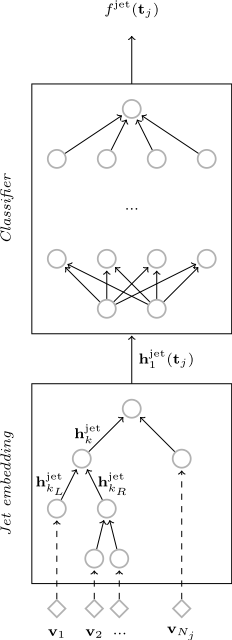
\includegraphics[width=\textwidth]{figures/qcd-rnn.png}
        \end{column}
    \end{columns}
\end{frame}

\begin{frame}
    \frametitle{Jet-level classification results}

    \begin{columns}
        \begin{column}{0.65\textwidth}
            {\scriptsize
            \begin{itemize}
                \item W-jet tagging example (data from \href{https://arxiv.org/abs/1609.00607}{1609.00607})
                \item On images, RNN has similar performance to previous CNN-based approaches.
                \item Improved performance when working with calorimeter towers, without image pre-processing.
                \item Working on truth-level particles led to significant improvement.
                \item Choice of jet algorithm matters.
            \end{itemize}}

            \centering
            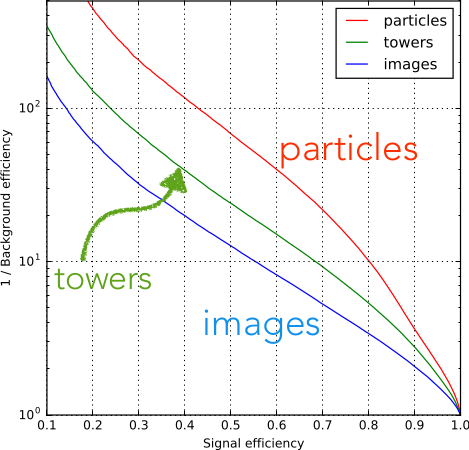
\includegraphics[width=0.6\textwidth]{figures/plot.png}
        \end{column}
        \begin{column}{0.35\textwidth}
            \centering
            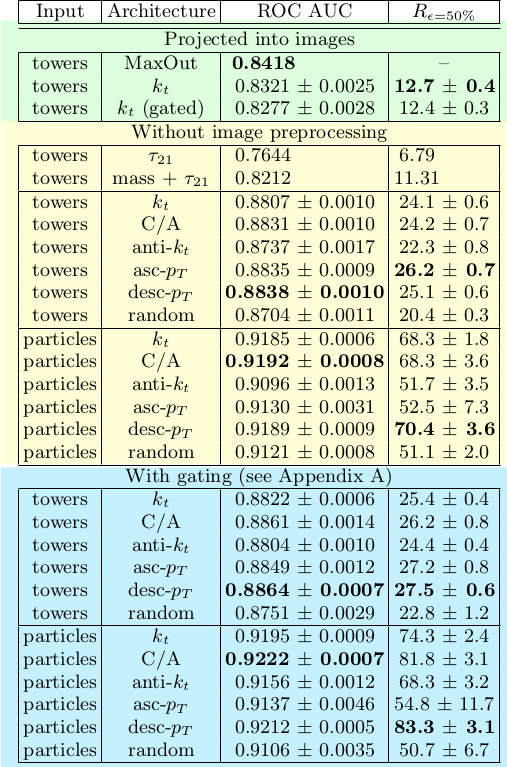
\includegraphics[width=1.1\textwidth]{figures/table.png}
        \end{column}
    \end{columns}
\end{frame}

\begin{frame}
    \frametitle{From paragraphs to events}

    \begin{center}
        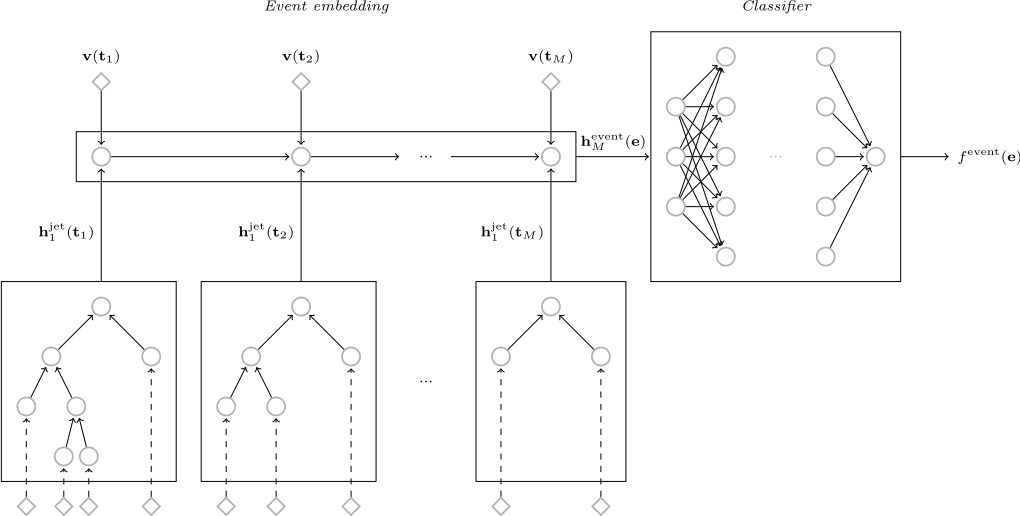
\includegraphics[width=\textwidth]{figures/event-rnn.png}
    \end{center}


    \begin{columns}
        \begin{column}{0.5\textwidth}
            Analogy:
            \begin{itemize}
                \item word $\rightarrow$ particle
                \item sentence $\rightarrow$ jet
                \item parsing $\rightarrow$ jet algorithm
                \item paragraph $\rightarrow$ event
            \end{itemize}
        \end{column}
        \begin{column}{0.5\textwidth}
            \centering
            {\color{red}Joint learning of jet embedding, event embedding and classifier.}
        \end{column}
    \end{columns}


\end{frame}

\begin{frame}
    \frametitle{Event-level classification results}

    \begin{columns}
        \begin{column}{0.6\textwidth}
            RNN on jet-level 4-momentum $v(t_j)$ only vs. adding jet-embeddings $h_j$:
            \begin{itemize}
                \item Adding jet embedding is much better (provides jet tagging information).
            \end{itemize}

            \vspace{0.5cm}

             RNN on jet-level embeddings vs. RNN that simply processes all particles in the event:
            \begin{itemize}
                \item Jet clustering and jet embeddings help a lot!
            \end{itemize}
        \end{column}
        \begin{column}{0.4\textwidth}
            \centering
            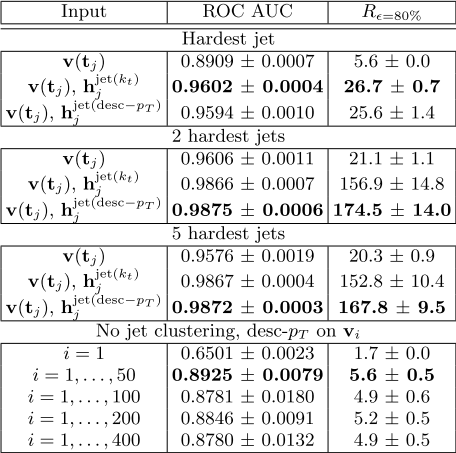
\includegraphics[width=\textwidth]{figures/table2.png}
        \end{column}
    \end{columns}
\end{frame}

\begin{frame}
    \frametitle{Summary}

    \begin{itemize}
        \item Neural networks are computational graphs whose architecture can be molded on a per-sample basis to express and impose domain knowledge.

        \item Our QCD-aware recursive net operates on a variable length set of 4-momenta and use a computational graph determined by a jet algorithm.

        \begin{itemize}
            \item Experiments show that topology matters.
            \item Alternative to image-based approaches.
            \item Requires much less data to train (10-100x less data).
        \end{itemize}

        \item The approach directly extends to the embedding of full events. Intermediate jet representation helps.

        \item Many more ideas of hybrids of QCD and machine learning!
    \end{itemize}

\end{frame}

\end{document}
